\section{\bf Modified Valiant's algorithm}

In this section we describe the reorganization of submatrix processing order in the Valiant's algorithm which simplify independent handling of submatrices. As a result, proposed modification can facilitate implementation of parallel submatrix processing.

\subsection{\bf \it Layered submatrices processing}

The main change of this modification is the possibility to divide the parsing table into layers of disjoint submatrices of the same size.
The idea of division we have made from the reorganization of the matrix multiplication order is presented in figure~\ref{fig2}.
Each layer consists of square matrices which size is power of 2.
The layers are computed successively in the bottom-up order.
Each matrix in the layer can be handled independently, which can help to implement parallel version of layer processing function.

\begin{figure}[h]
\vspace{3mm}
 \begin{center}
 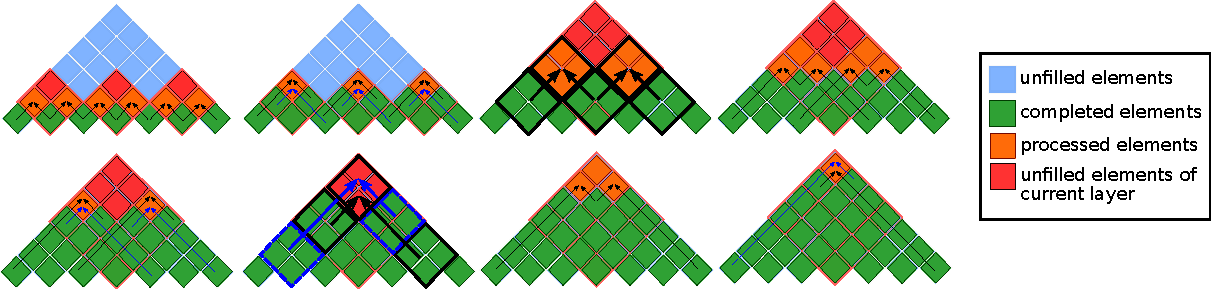
\includegraphics[width=12cm]{pictures/modivis2.pdf}
    \caption{An example of the modification of Valiant's algorithm}
    \label{fig4}
 \end{center}
\vspace{-8mm}
\end{figure}

A simple example of the modification is shown in figure~\ref{fig4}.
The lowest layer (submatrices which size is 1) is already computed and filling of the matrix starts with the second layer (subfigures 1-2).
Note that the same  process is presented in figure~\ref{fig3}, but here it can be done only in two steps using parallel computation of submatrix products.

The modified version of Valiant's algorithm is presented in listing~\ref{algo:modified}.
The procedure \textit{main()} computes the lowest layer $(T_{l, l+1})$, and then divide the table into layers, described earlier, and computes them through the \textit{completeVLayer()} call.
Thus, \textit{main()} computes all elements of parsing table $T$.
(Hereinafter, we use layer to mean set of submatrices.)

For brevity, we define \textit{left(subm), right(subm), top(subm), bottom(subm), \linebreak rightgrounded(subm)} and \textit{leftgrounded(subm)} functions which returns the submatrices for matrix $subm = (l, m, l', m')$ according to the original Valiant's algorithm (figure~\ref{fig2}).

Also denote some subsidiary functions for matrix layer $M$:
\begin{itemize}[noitemsep, nolistsep]
    \item[$-$] \textit{bottomsublayer(M)} $ = \{bottom(subm)\, |\,subm \in M \}$,
    \item[$-$] \textit{leftsublayer(M)} $ = \{\textit{left(subm)}\, |\,subm \in M \}$,
    \item[$-$] \textit{rightsublayer(M)} $ =\{\textit{right(subm)}\, |\,subm \in M \}$,
    \item[$-$] \textit{topsublayer(M)} $ = \{top(subm)\, |\,subm \in M \}$.
\end{itemize}

\begin{algorithm}[!h]
\SetAlgoNoLine
\KwIn{$G = (\Sigma, N, R, S), w = a_{1} \dots a_{n}, n \geq 1, n + 1 = 2^p, a_{i} \in \Sigma$ }
\underline{main()}{:}{

 \For {$l \in \{1, \ldots, n \}$}{$T_{l, l + 1} = \{A | A \rightarrow a_{l + 1} \in R\}$}
 \For{$1 \le i < p - 1 $}{
 layer = \textit{constructLayer(i)}\;
 \textit{completeVLayer(layer)}
 }
 accept if and only if $S \in T_{0, n}$
 \BlankLine
 }

\underline{constructLayer(i)}{:}{
 \BlankLine
 $\{(k2^i, (k+1)2^i, (k + 1)2^i, (k+2)2^i) \, |\, 0 \le k < 2^{p - i} - 1\}$
 \BlankLine
    }
\underline{completeLayer(M)}{:}{
\BlankLine
\If {$\forall (l, m, l', m') \in M \quad (m - l = 1)$}{\For{$ (l, m, l', m') \in M$}{$T_{l, l'} = f(P_{l, l'})$\;}}
\Else{
\textit{completeLayer(bottomsublayer(M))}\;
\textit{completeVLayer(M)}
}
\BlankLine
}

\underline{comleteVLayer(M)}{:}{
 \BlankLine
 \textit{multiplicationTasks$_1$ = \linebreak
    \{$left(subm)$, $leftgrounded(subm)$, $bottom(subm)\, |\,subm \in M \} \cup \linebreak  \{right(subm), bottom(subm), rightgrounded(subm)\, |\,subm \in M\}$\;}
 \BlankLine
 multiplicationTask$_2$ = $\{top(subm), leftgrounded(subm), right(subm)\, |\,subm \in M\}$\;
 \BlankLine
 multiplicationTask$_3$ = $\{top(subm), left(subm), rightgrounded\, |\,subm \in M\}$\;
 \BlankLine
 \textit{performMultiplications(multiplicationTask$_1$)}\;
 \textit{completeLayer(leftsublayer(M) $\cup$ rightsublayer(M))}\;
 \textit{performMultiplications(multiplicationTask$_2$)}\;
 \textit{performMultiplications(multiplicationTask$_3$)}\;
 \textit{completeLayer(topsublayer(M))}

 }
 \BlankLine

 \underline{performMultiplication(tasks)}{:}{\\
 \For{$ (m, m1, m2) \in \textit{tasks}$}{$P_{m} = P_{m} \cup (T_{m1} \times T_{m2})$\;}
 }

\caption{Parsing by matrix multiplication: Modified Version}
\label{algo:modified}
\end{algorithm}


The procedure \textit{completeVLayer(M)} takes an array of disjoint submatrices $M$ which represents a layer.
For each \textit{subm = (l, m, l', m') $\in M$} this procedure computes \textit{left(subm), right(subm), top(subm)}.
The procedure assumes that the elements of \textit{bottom(subm)} and $T_{i, j}$ for all $i$ and $j$ such that $l \leq i < j < m$ and $  l' \leq i < j < m'$ are already constructed.
Also it is assumed that the current value of
$P_{i, j} =  \{ (B, C) | \exists k, (m \le k < l'), a_{i + 1} \dots a_{k} \in L_G(B), a_{k + 1} \dots a_{j} \in L_G(C)\} $ for all $i$ and $j$ such that $l \leq i < m$ and $l' \leq j < m'$.

The procedure \textit{completeLayer(M)} also takes an array of disjoint submatrices $M$, but unlike the previous one, it computes $T_{i, j}$ for all $(i, j) \in subm$.
This procedure requires exactly same assumptions on $T_{i, j}$  and $P_{i, j}$  as in the previous case.

In the other words, \textit{completeVLayer(M)} computes the entire layer \textit{M} \linebreak and \textit{completeLayer($M_{2}$)} is a support function which is necessary for computation of smaller square submatrices $subm_{2} \in M_{2}$ inside of \textit{M}.

Finally, the procedure \textit{performMultiplication(tasks)}, where \textit{tasks} is an array of a triple of submatrices, perform basic step of algorithm: matrix multiplication. It is worth mentioning that, as distinct from the original algorithm, here $|tasks| \ge 1$ and each task can be computed independently.
So, practical implementation of this procedure can easily involve different techniques of parallel array processing, such as OpenMP~\ref{!!!}.

\subsection{\bf \it Algorithm for substrings}

Next we show how our modification can be applied to the string-matching problem.

So if we want to find all substrings of size $s$ which can be derived from a start symbol for an input string of size $n = 2^p$, we need to compute layers with submatrices of size not greater than $2^{l'}$, where $2^{l' - 2} < s \le 2^{l' - 1}$.

Let $l' = p - (m - 2)$ and consequently $(m - 2) = p - l'$.

For any  $m \le i \le p$ products of submatrices of size $2^{p - i}$ are calculated exactly $2^{2i - 1} - 2^{i}$ times and each of them imply multiplying $\mathcal{O}(|G|)$ Boolean submatrices.

\begin{equation}
\begin{array}{c}
C \sum\limits_{i=m}^p 2^{2i - 1} \cdot 2^{\omega(p - i)} \cdot f(2^{p - i}) =
C \cdot 2^{\omega l'}\sum\limits_{i=2}^{l'} 2^{(2 - \omega)i} \cdot 2^{2(p - l') - 1} \cdot f(2^{l' - i}) \le \\
C \cdot 2^{\omega l'} f(2^{l'}) \cdot 2^{2(p - l') - 1} \sum\limits_{i=2}^{l'} 2^{(2 - \omega)i} =
BMM(2^{l'}) \cdot 2^{2(p - l') - 1} \sum\limits_{i=2}^{l'} 2^{(2 - \omega)i}
\end{array}
\end{equation}

Thus, time complexity for searching all substrings is  $O(|G|BMM(2^{l'})(l' - 1))$, while time complexity for the full input string is $O(|G|BMM(2^p)(p - 1))$. In contract to the modification, Valiant's algorithm completely calculate at least 2 triangle submatrices of size $\frac{n}{2}$ (as shown in figure~\ref{fig5}) which mean minimum asymptotic complexity  $O(|G|BMM(2^{p - 1})(p - 2))$. Make a conclusion that the modification is asymptotically faster for substrings of size $s \ll n$  than the original algorithm.

\begin{figure}[h]
\vspace{3mm}
 \begin{center}
 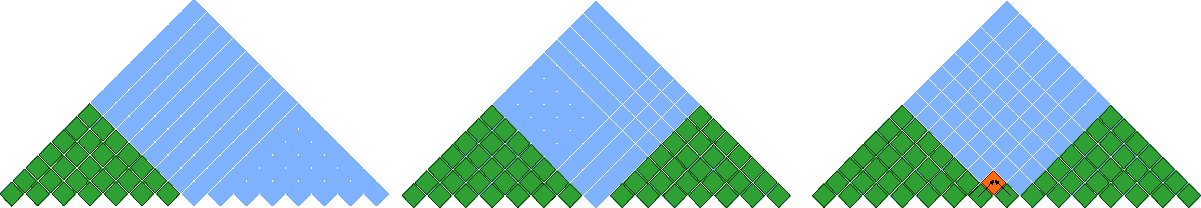
\includegraphics[width=12cm]{pictures/valsubstring.pdf}
    \caption{The number of elements necessary to compute in Valiant's algorithm. That means it is nessesary to calculate at least 2 triangle submatrices of size $\frac{n}{2}$.}
    \label{fig5}
 \end{center}
\vspace{-8mm}
\end{figure}
